\documentclass[12 pt]{article}
\usepackage[utf8]{inputenc}
\usepackage{graphicx}
\usepackage{amsmath}
\usepackage{amssymb}
\usepackage{multirow}
\usepackage{caption}
\usepackage{subcaption}
\usepackage{hyperref}
\usepackage{pgf}
\usepackage{pgfpages}
\usepackage{textcomp}
\usepackage{lscape}
\usepackage{geometry}
\usepackage{pdflscape} 
\usepackage{placeins}
\usepackage{url}
\usepackage{natbib}
\usepackage[paper=A4]{typearea}
\graphicspath{ {figures/} }
\usepackage{array}
\usepackage{bookmark}% faster updated bookmarks
%\usepackage[a4paper,margin=1in]{geometry}



\pgfpagesdeclarelayout{boxed}
{
  \edef\pgfpageoptionborder{0pt}
}
{
  \pgfpagesphysicalpageoptions
  {%
    logical pages=1,%
  }
  \pgfpageslogicalpageoptions{1}
  {
    border code=\pgfsetlinewidth{2pt}\pgfstroke,%
    border shrink=\pgfpageoptionborder,%
    resized width=.95\pgfphysicalwidth,%
    resized height=.95\pgfphysicalheight,%
    center=\pgfpoint{.5\pgfphysicalwidth}{.5\pgfphysicalheight}%
  }%
}

\pgfpagesuselayout{boxed}

\title{Assignment 1}
\author{Abhijeet Mangela}
\date{November 2022}

\title{Assignment 1}
\author{Abhijeet Mangela}
\date{\today}

\begin{document}
\begin{titlepage}
\begin{center}

\textbf{\huge Design project report Group 7 \\ \vspace{0.4 cm} Week 3} \\

\vspace{2 cm}

\centering

\includegraphics[width=0.5\textwidth]{IIT_Madras_Logo.svg.png}
\label{fig:my_label}

\vspace{1cm}

\textbf{Abhijeet Mangela AE21B040 \\ Navin Yadav AE23M803 \\ Balamurugan S AE23M009 \\ Samarth R Krishna AE23M032 \\ Senthil B AE23M035 \\ Rajendran Anandhu Nair AE23M027 }

\vspace{0.5cm}

\footnotesize Department of Aerospace Engineering \\
IIT Madras \\
India

\normalsize

\end{center}
\end{titlepage}


\newpage

\tableofcontents

\newpage

\thispagestyle{empty}
\listoffigures
\listoftables
\newpage


\section{Introduction}

\subsection{Objective}
The primary objective of this design project is to design and fly a fixed-wing UAV that can survey wildlife and monitor plastic-free zones/environments in amusement parks, zoos, and wildlife sanctuaries.


\subsection{Abstract}
Air quality is an essential measure of the quality of life of any living being. A decrease in air quality is easily linked with a reduction in the life expectancy of various plants and animals.

As a result, we are focused on working on a drone that will give us an insight into the air quality of a region. 

We often have to measure air quality within a forest or a region where it is hard to go physically. As a result, we have to place expensive monitoring sensors at various challenging-to-reach locations. 

When some maintenance issues arise in these sensors, we again have to send teams to repair the equipment.

These complications can be reduced by using a fixed-wing UAV instead of ground sensors because the UAV is a moving object that can cover a larger area than a UAV sensor alone. Also, if some maintenance problem arises, it can be fixed when the UAV lands.

The UAV will also visually surveillance the land it is flying. A direct flight will provide a better and more frequent information intake than satellite imagery.

\subsection{Mission Profile and requirements}

\subsubsection{Mission Requirement}
%Our objective is to detect the gases present near the airplane. It should detect elements including PM2.5, PM10, O3, NO2, SO2, CO, VOCs, H2S, NH3, HCl, CxHy, H2 and more.
In a crowd gathering, ensuring the cleanliness of a natural environment conducive to the dwelling of fauna is challenging. To overcome this problem steadfastly without affecting the crowd's morale, instead of acting as an entertainment element in satisfying the objective above, UAVs are identified as the best choices amidst these situations. 


The UAV will be equipped with air quality sensors and cameras to understand the terrain better. Thus, knowledge about plastics and unpleasant atmospheres will help develop a quick action plan for maintaining the flora and fauna from foreign hazards.

\subsubsection{Aircraft Characteristics}
\begin{table}[h]
\centering
\resizebox{0.55\textwidth}{!}{%
\begin{tabular}{|c|c|}
\hline
\textbf{Estimated MTOW}            & 8 – 10 kg                \\ \hline
\textbf{Maximum Payload Weight}    & 1 – 1.5 kg               \\ \hline
\textbf{Estimated Endurance}       & 30 minutes               \\ \hline
\textbf{Mission ceiling}           & 0 - 250 m                \\ \hline
\textbf{Desired Operational Speed} & 17 m/s                   \\ \hline
\textbf{Transmitter Range}         & 4 km                     \\ \hline
\end{tabular}%
}
\caption{Initial Mission Requirements}
\label{Mission Requirements}
\end{table}

\subsubsection{Payload measure}
The payload of UAVs consists of a camera and a sensor module used to measure air quality. The camera will be a Hontral B0BMV12VYJ HD Camera weighing 492 g. The sensor module comprises Arduino MKR Proto Large Shield TSX00002, weighing about 200 g, and sensors such as MQ-7 CO Carbon Monoxide, MG811 Air Carbon Dioxide, etc., weighing about 320 g.

\subsection{Mission Profile}

\begin{figure}[h]
    \centering
    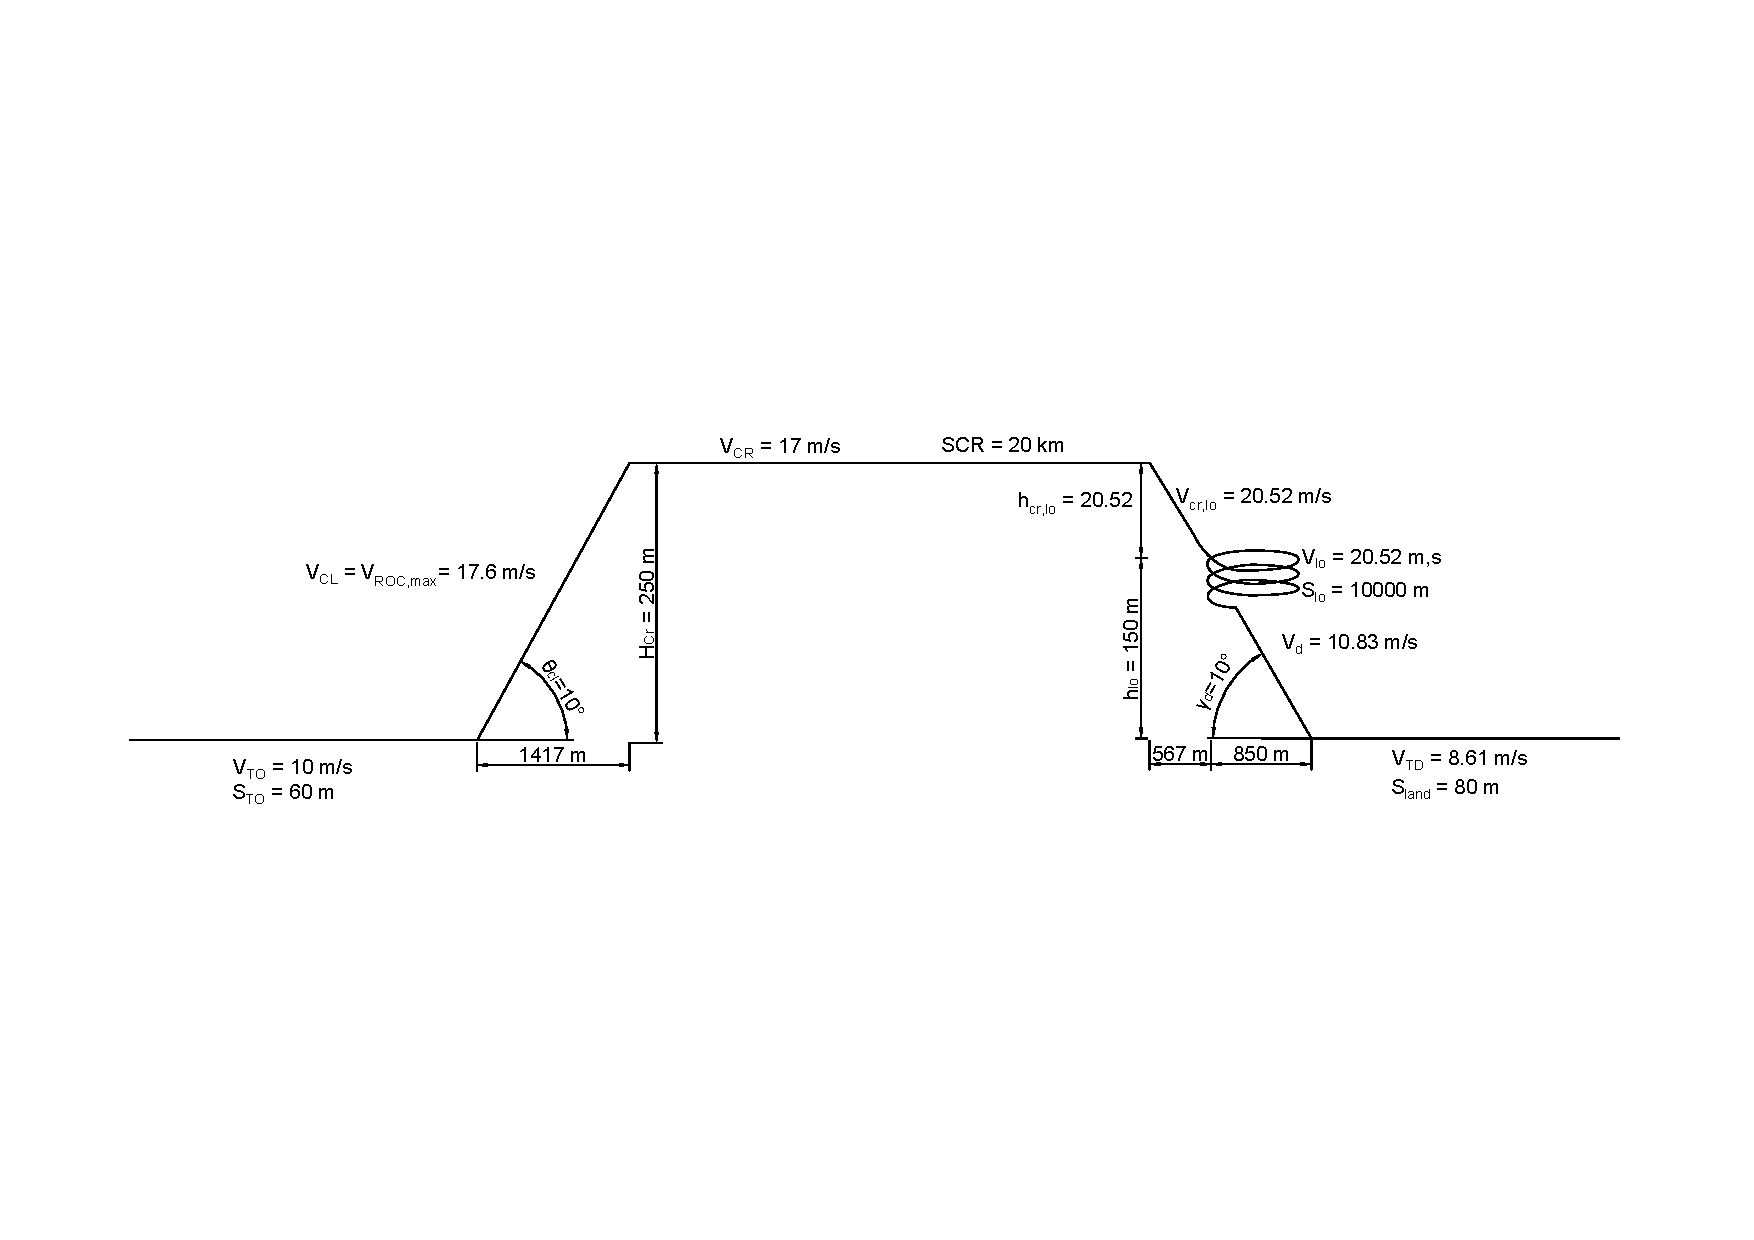
\includegraphics[width = \linewidth]{Drawing1-Model_final.pdf}
    \caption{Mission Profile}
    \label{Mission Profile}
\end{figure}


\subsubsection{Ground run}
The take-off ground run distance is approximately 60 meters, and the estimated take-off velocity is ten m/s. \cite{EgglestonUnknownTitle2015}

$$ (V_{TO})_{_{Bricans \: Td100}} = 19 \: m/s$$
$$ (W_{TO})_{_{Bricans \: Td100}} = 22.67 \: kg$$

Since $ V_{TO} \: \alpha \: \sqrt{W_{TO}} $ for given $C_L$ , S (applicable for initial estimate)

$$ (V_{TO})_{_{des}} = (V_{TO})_{_{Bricans \: Td100}} \times \sqrt{\frac{(W_{TO})_{_{des}}}{(W_{TO})_{_{Bricans \: TD \: 100}}}} $$

$$ = 19 \times \sqrt{\frac{5.6 \times 9.81}{22.67 \times 9.81}} = 9.94 \: m/s \approx 10 \: m/s $$

\subsubsection{Climb \cite{1000_questions} }
The UAV will climb at an estimated velocity of 17.6 m/s to an operating altitude of 250 m AMSL. The rate of climb is about 3.06 m/s. Time spent here: 81.7 s

Calculation :- 
$$ (V_{TO})_{_{des}} = 10 \: m/s \Rightarrow (V_{stall})_{_{des}} = \frac{(V_{TO})_{_{des}}}{1.2} = 8.33 \: m/s $$
$$ (V_{md})_{_{des}} = 1.6 \times V_{stall} = 13.33 \: m/s $$
$$ (V_{ROC})_{_{max}} = 1.32 \times V_{md} = 17.6 \: m/s $$

\subsubsection{Cruise \cite{alhajjaji2017design}}
The UAV will perform aerial surveillance and environmentally monitor for areas of plastics and solid waste with an estimated cruise speed of 17 m/s for the 20 km range. Time spent here is 1176 s.

\subsubsection{Descent to Mission Height}
The UAV will descend to an altitude of 150 m AMSL to study air quality at a sinking speed of 12.92 m/s for a 5 km range. Time spent here is 28 s.\\

Calculation: - 
$$ (V_{cr,lo})_{_{design}} = 0.76 \times (V_{cr})_{_{des}} \;  (initial \: estimate) $$
$$ = 12.92 \: m/s $$

\subsubsection{Descent to land \cite{Anderson1}}
The UAV will descend at an estimated velocity of 10.13 m/s. To close ground proximity, the UAV gradually decelerates to an estimated touchdown velocity of 8.61 m/s. Time spent here is 80 s.
Calculation: - 
$$(V_des)_{_{design}} = (V_{mg})_{_{design}} = (V_{mg})_{_{design}} \times 0.76 = 10.13 \: m/s $$

\subsubsection{Landing run}
The landing ground run distance is approximately 80 metres, and the estimated touchdown velocity is 8.61 m/s.

Calculation: - 
$$ (V_{TD})_{_{design}} = 0.85 \times (V_{des})_{_{design}} = 8.61 \: m/s  $$
$$ \text{Vertical component of } (V_{TD})_{_{design}} = 8.61 \times \sin{10^{\circ}} $$
$$ = 1.495 \: m/s \leq 4 \: m/s \; \text{(For smooth landing)} $$



\subsection{Data collection}

The data of all the parameters:-
% Please add the following required packages to your document preamble:
% \usepackage{graphicx}
\begin{table}[h]
\centering
\resizebox{\textwidth}{!}{%
\begin{tabular}{|c|c|c|c|c|c|c|c|}
\hline
SI no &
  UAV Name &
  \begin{tabular}[c]{@{}c@{}}MTOW \\ Kg\end{tabular} &
  \begin{tabular}[c]{@{}c@{}}Empty Weight\\ kg\end{tabular} &
  \begin{tabular}[c]{@{}c@{}}Battery Weight\\ kg\end{tabular} &
  \begin{tabular}[c]{@{}c@{}}Payload Weight\\ kg\end{tabular} &
  \begin{tabular}[c]{@{}c@{}}Range \\ km\end{tabular} &
  \begin{tabular}[c]{@{}c@{}}Endurance\\ min\end{tabular} \\ \hline
1 & Wingtraone   \cite{Wingtra}             & 4.5 & 2.387 & 0.604       & 1.509 &     & 59  \\ \hline
2 & Albatross    \cite{Albatross}             & 10  & 3.5   & 2.4         & 4.1   & 250 & 240 \\ \hline
3 & Azimut   2    \cite{Azimut}            & 9   & 2.5   & 2.8         & 3.7   &     &     \\ \hline
4 & Dragonfly   Tango 2  \cite{Dragonfly}      & 5   & 3     & 0.595+0.595 & 1.5   & 5   & 120 \\ \hline
5 & Nostromo   Defensa Cabure \cite{Nostromo} & 5   & 3.4   & 0.604       & 1     & 15  & 1.5 \\ \hline
6 & SPY   LITE    \cite{Bluebird}            & 9.5 & 4.5   & 1.5         & 1.35  & 80  & 240 \\ \hline
7 & Skylark I-LEX   \cite{Skylark}          & 7.5 & 5.5   & 0.8         & 1.2   & 40  & 180 \\ \hline
\end{tabular}%
}
\caption{Data part one}
\label{Data part one}
\end{table}

% Please add the following required packages to your document preamble:
% \usepackage{graphicx}
\begin{table}[h]
\centering
\resizebox{\textwidth}{!}{%
\begin{tabular}{|c|c|c|c|c|c|c|c|c|c|}
\hline
SI no &
  UAV Name &
  \begin{tabular}[c]{@{}c@{}}Service Ceiling\\ m\end{tabular} &
  \begin{tabular}[c]{@{}c@{}}Maximum Ceiling\\ m\end{tabular} &
  \begin{tabular}[c]{@{}c@{}}Cruise speed\\ km/hr\end{tabular} &
  \begin{tabular}[c]{@{}c@{}}Max Speed\\ km/hr\end{tabular} &
  \begin{tabular}[c]{@{}c@{}}Longitudinal Length\\ cm\end{tabular} &
  \begin{tabular}[c]{@{}c@{}}Wing Span\\ cm\end{tabular} &
  AR &
  L/D \\ \hline
1 & Wingtraone                & 120  & 2500   to 5000 & 35.8 &     &     & 125 & 1.838 &                \\ \hline
2 & Albatross                 &      &                & 68   & 129 &     & 300 &       & 28:1   to 30:1 \\ \hline
3 & Azimut   2                &      &                &      &     &     &     &       &                \\ \hline
4 & Dragonfly   Tango 2       &      &                & 43.2 & 100 &     &     &       &                \\ \hline
5 & Nostromo   Defensa Cabure & 4000 &                & 70   & 105 &     &     &       &                \\ \hline
6 & SPY   LITE                &      &                &      & 120 & 135 & 275 &       &                \\ \hline
7 & Skylark I-LEX             & 4572 &                & 37   & 74  & 220 & 300 &       &                \\ \hline
\end{tabular}%
}
\caption{Additional data}
\label{Data part 2}
\end{table}


\begin{figure}[h!]
    \begin{subfigure}{.4\textwidth}
        \centering
        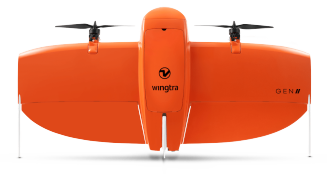
\includegraphics[width = 0.8\linewidth]{Aircraft pics/WingtraOne.png}
        \caption{Wingtraone}
        \label{Wingtra one}
    \end{subfigure}
    \begin{subfigure}{.4\textwidth}
        \centering
        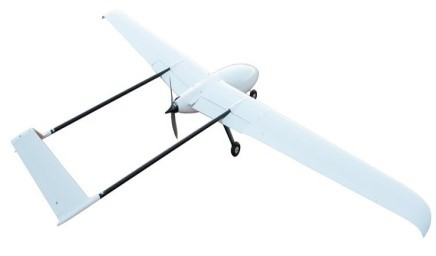
\includegraphics[width = 0.8\linewidth]{Aircraft pics/Albatross.jpg}
        \caption{Albatross}
        \label{Albatross}
    \end{subfigure}
    \begin{subfigure}{.4\textwidth}
    \centering
    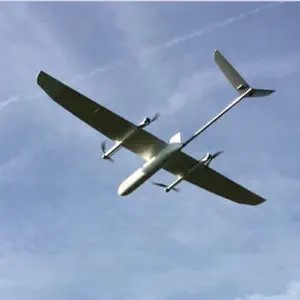
\includegraphics[width=0.8\linewidth]{Aircraft pics/Azimut.jpg}
    \caption{Azimut 2}
    \label{Azimut 2}
    \end{subfigure}
    \begin{subfigure}{.4\textwidth}
        \centering
        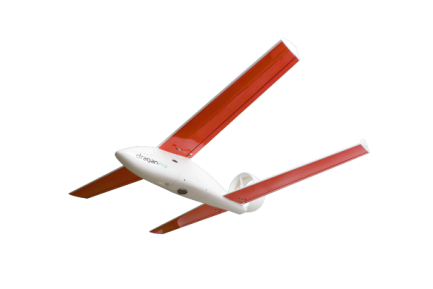
\includegraphics[width = 0.8\linewidth]{Aircraft pics/Dragonfly.png}
        \caption{Dragonfly Tango 2}
        \label{Dragonfly Tango 2}
    \end{subfigure}
    \begin{subfigure}{.4\textwidth}
        \centering
        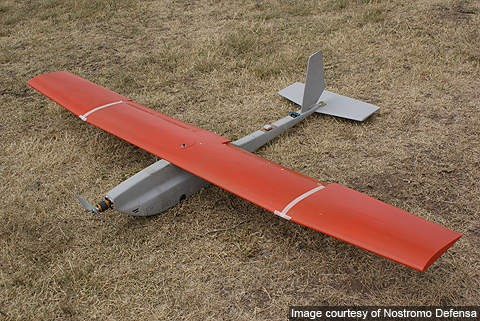
\includegraphics[width = 0.8\linewidth]{Aircraft pics/Nostroma.jpg}
        \caption{Nostroma Defensa Cadambra}
        \label{Nostromo Defence Cadambra}
    \end{subfigure}
    \begin{subfigure}{.4\textwidth}
        \centering
        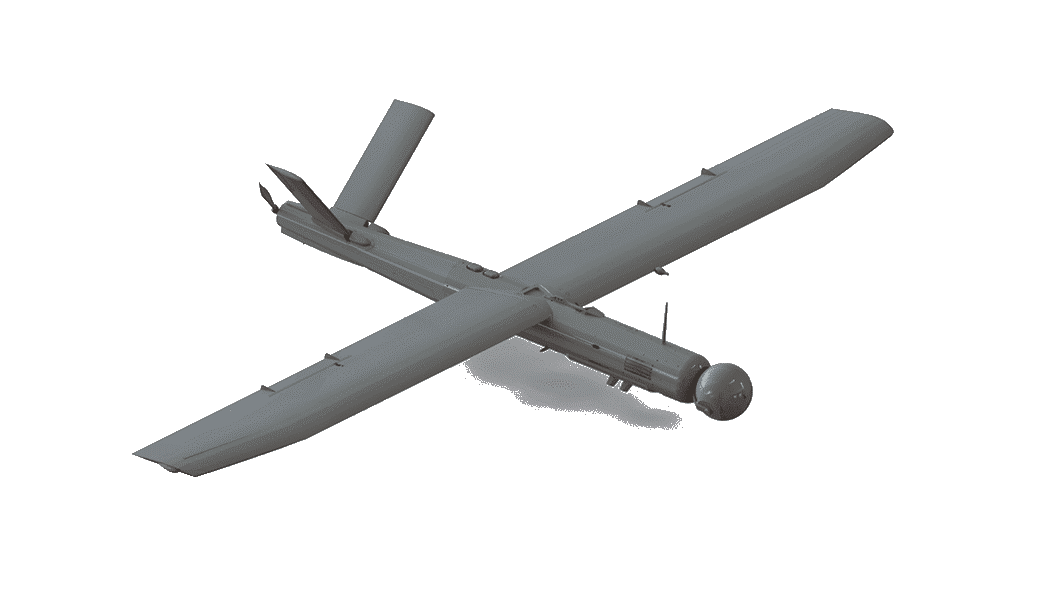
\includegraphics[width = 0.8\linewidth]{Aircraft pics/spylite.png}
        \caption{Spylite}
        \label{Spylite}
    \end{subfigure}
    \centering
    \begin{subfigure}{.4\textwidth}
        \centering
        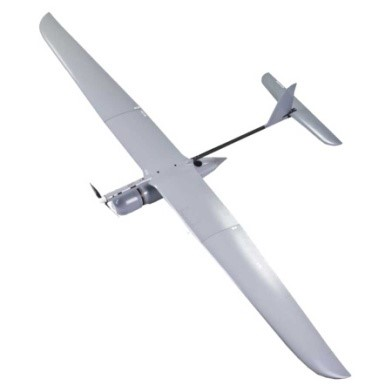
\includegraphics[width = 0.8\linewidth]{Aircraft pics/Skylark.jpg}
        \caption{Skylark}
        \label{Skylark}
    \end{subfigure}
    \caption{List of drones studied}
    \label{Drone pictures}
\end{figure}


\vspace{\fill}

\newpage


%\Floatbarrier
%\vspace{\vfill}

\section{Preliminary Weight estimation}

Weight estimation is divided into various sections
\subsection{Payload weight estimation}
Rough estimate for payload
\begin{table}[h]
\centering
\resizebox{0.6\textwidth}{!}{%
\begin{tabular}{|c|c|}
\hline
Purpose                            & Weight \\ \hline
Camera                             & 492 g  \\ \hline
Sensor module                      & 520 g  \\ \hline
Bulk Tolerance (Wiring, Actuation) & 388 g  \\ \hline
Total Payload Estimate             & 1400 g \\ \hline
\end{tabular}%
}
\caption{Payload weight estimate}
\label{Payload weight}
\end{table}

\hfill


\subsection{Empty weight estimation}
The empty weight ratio can be estimated from the previous data. We have to fit the data in the $y = A x^c$ curve with A and C as variables.

In our Data, A is 1.3887, and C is -0.5155

\begin{figure}[h]
    \centering
    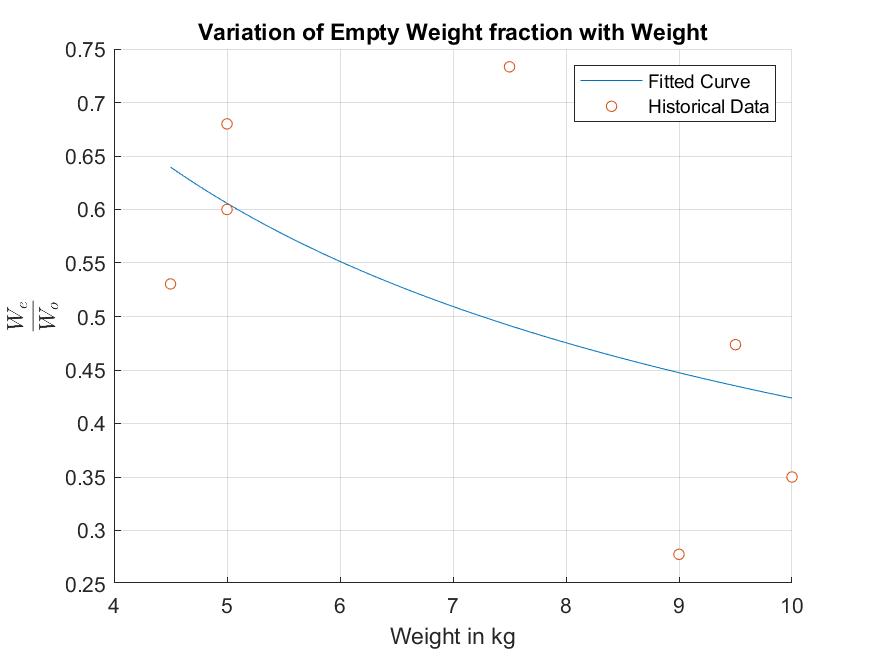
\includegraphics[width = 0.8\linewidth]{Codes/Week 2/Empty_weight.png}
    \caption{Empty weight estimation}
    \label{Empty Weight estimation}
\end{figure}

The empty weight in our drone came out to be 3.1746 kg.

\newpage

\subsection{Battery weight estimation}

The battery is an essential criterion for the design of any drone. We should optimize the battery weight using the Mission profile we have. That way, we will not be carrying unnecessary dead weight with us.

For calculating Battery weight estimation, we must first find out the total energy required for each Major phase of flight.

\subsubsection{Cruise}
Now, for a level flight,
$$ L = W \; \; , \; \; T = D$$

$$ W = \frac{1}{2} \rho V^2 S C_L $$
$$ C_L = \frac{W}{\frac{1}{2} \rho V^2 S}$$
So,
$$ C_D = C_{D_0} + \frac{C_L^2}{\pi e AR} $$
Now 
$$ P = T\times V = D\times V $$

So, 
$$ P_R = \frac{1}{2}\rho V^3 S C_{D_o} + \frac{2 W^2}{ (\rho V S) \pi e AR} $$

$$P_R = f(W,\rho,V,C_{D_o},S,e,AR)$$

Taking approximations and inputting mission profile conditions

$$ P_R = f(W) $$

We will consider the Loitor phase as a cruise, too.

For our cruise phase of 17 m/s, we will need a power of 63.42 W.

\subsubsection{Climb }
The power required for climb is given by 
$$ P = W \times R.O.C + P_R $$

Climbing is also the portion where we need a good amount of power. For our estimated weight, we need a preliminary power of 87 W.

\subsubsection{Descent}
The power required for descent is 
$$ P = P_R - W \times Rate\: of\: descent$$
We need to ensure the power does not go negative here or make it zero while estimating energy. The extra allowance we give will take care of the power consumed.

\subsubsection{Take off and Landing}
The Segments of take-off and Landing do not take that much time. Also, estimating the energy spent in takeoff and Landing is harder due to the carrying power needs. So, we will take an excess power of 20 percent to account for the errors in different power situations.

\subsubsection{Battery type selection \cite{Lipobattery}}

We will use a lithium polymer battery for our aircraft. Some of the advantages offered by a lithium polymer battery are that it is less likely to leak away and still rivals Lithium-ion batteries in terms of energy density. It is bulkier by volume, but by weight, it is comparable.

\begin{figure}[h]
    \centering
    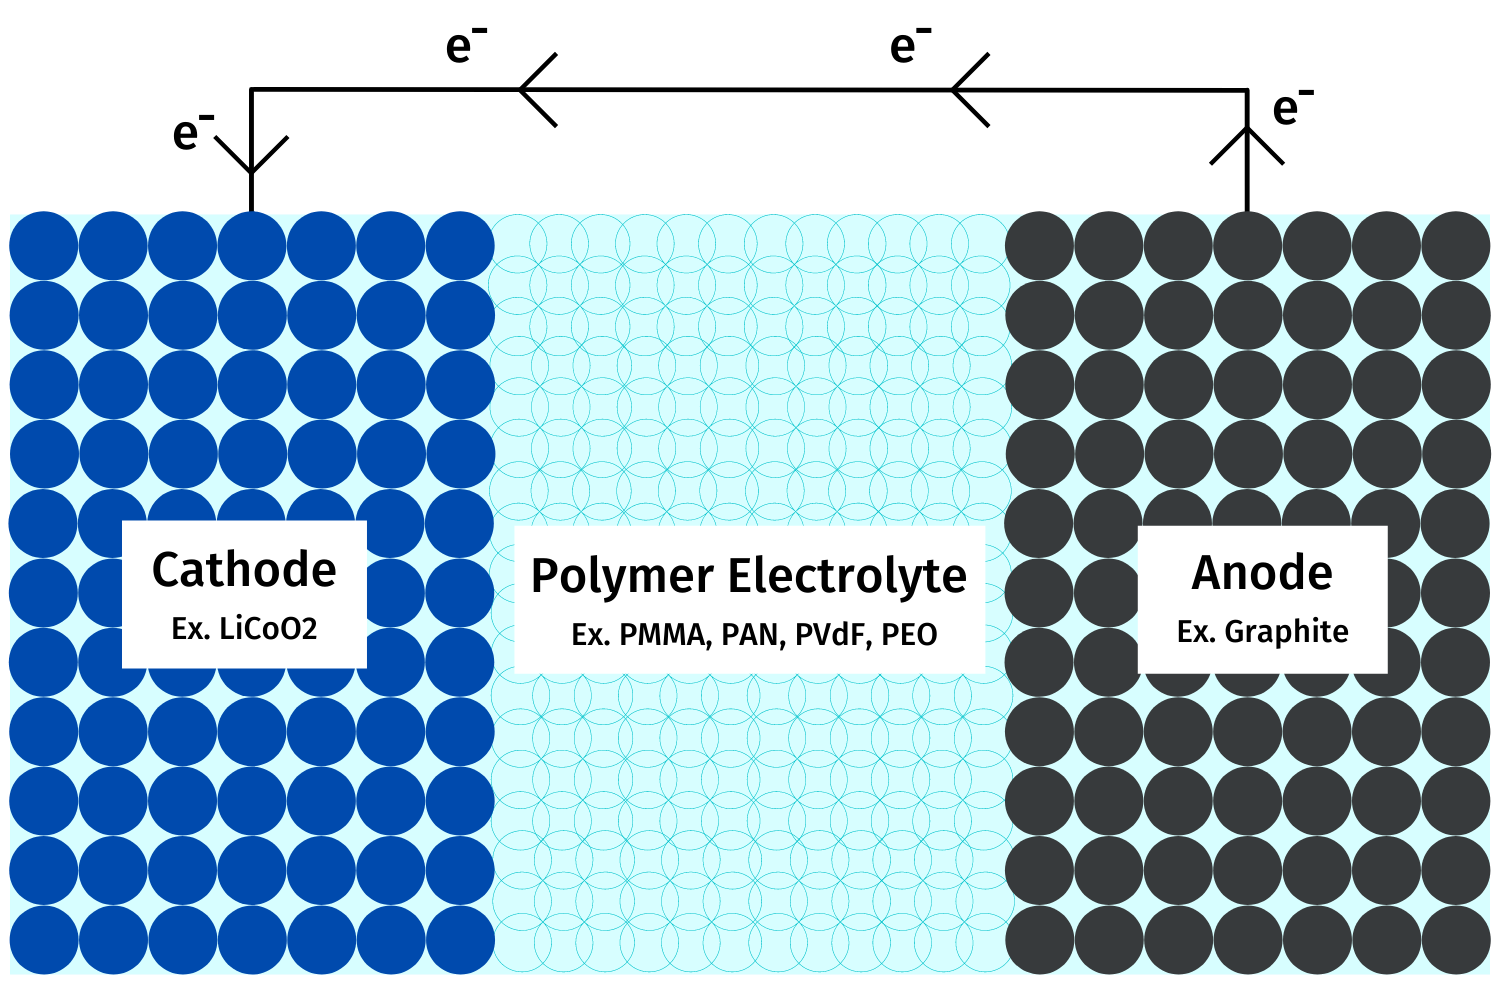
\includegraphics[width=0.5\linewidth]{Extra pics/LiPo_battery_diagram.png}
    \caption{Lithium Polymer battery}
    \label{Lithium Polymer battery}
\end{figure}

Lithium Polymer batteries are rechargeable batteries that transmit electricity due to the difference in charge between the Cathode and Anode parts of the battery. While pretty safe to handle, care should be taken not to get the battery near any fore source, or else it tends to catch fire.

We can estimate the energy in a battery by using this formula \cite{Lipobattery}:-

$$ \text{Battery Capacity} = \sigma \times \text{M}_\text{battery} $$

We used a commercially available battery to calculate the battery energy density of it \cite{Batteryref}. The energy density came out to be 237600 J/kg.

\subsubsection{Battery weight}

We can calculate the energy by multiplying the power required by the time spent in that phase. From energy, we can get battery weight by dividing it by energy density. 

In our case, the battery weight came out to be 0.933 kg.

%For lithium polymer batteries, the energy density is around 273600.

\subsection{Total weight estimation}

The total weight is given as:- 
$$ W_0 = W_{pl} + W_{e} + W_{f} $$
Where,
\begin{itemize}
    \item[-] $W_0$ is the total design weight.
    \item [-] $W_{pl}$ is the payload weight.
    \item [-] $W_{e}$ is the empty weight.
    \item [-] $W_{f}$ is the fuel weight (Battery in our case).
\end{itemize}

It can be transformed into:- 
$$W_{0} = \frac{W_{pl}}{1 - \frac{W_{e}}{W_{0}} - \frac{W_{f}}{W_0}}$$

If we have an initial approximation, we can run an iteration algorithm to determine the design weight when we keep the empty weight ratio as a variable.

%Generally, we take an initial estimate to be four times the payload weight. Taking the correct initial weight is important,, or the code may blow up.

In our case, we use a special algorithm to preserve the momentum of the descent from the previous iteration. This is done because otherwise, the code will blow up and reach a negative value. 

$$ W_o = W_{\text{Previous iteration}} + W_{\text{New iteration}} $$

The code for the algorithm is mentioned below in the GitHub reference.

In our case, the design weight was 6.6102 kg after taking a 20 percent leverage over the original weight.

\begin{figure}
    \centering
    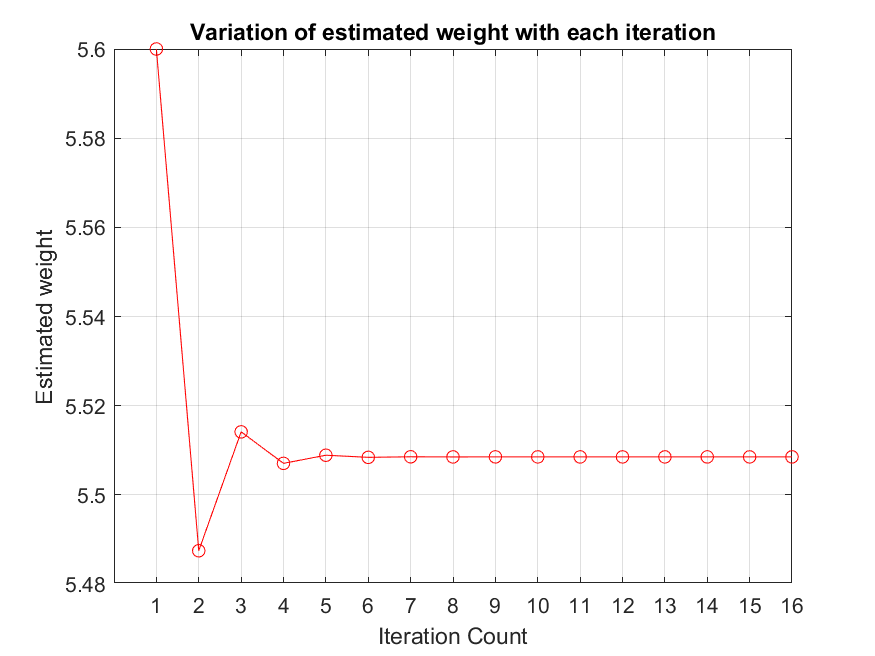
\includegraphics[width=0.75\linewidth]{Codes/Week 2/weight.png}
    \caption{Weight Estimation}
    \label{Weight Estimation}
\end{figure}

\vfill

\newpage

\section{Powerplant and Battery Selection}

\subsection{\ Extensive Calculation of Aspect Ratio and Lift Coefficient}

For this week, we first started by calculating the wing reference area and wetted area of all our reference UAVs and then proceeded to calculate the reference aspect ratio as well as the wetted aspect ratio of all the UAVs. We have used ImageJ and Fusion 360 software for estimating the Reference area and wetted area of all the UAV We \\
 The aspect ratio of a UAV's wings is crucial as it directly influences its aerodynamic performance and efficiency. Higher aspect ratios generally result in lower induced drag and better lift-to-drag ratios, enabling improved endurance and range, essential factors in UAV design optimization.
\\ The aspect ratio ($AR$) of a rectangular wing aircraft is calculated using the formula:
\[
AR = \frac{{\text{Wingspan}}}{{\text{Mean aerodynamic chord}}}\]

Where Wingspan is the distance between the wingtips and the Mean aerodynamic chord is the average chord length of the wing.

By using steady-level conditions where Lift = Weight, we have calculated the Lift Coefficient at cruise conditions.

When the lift force ($L$) of an aircraft equals its weight ($W$), the coefficient of lift ($C_L$) can be calculated using the formula:

\[
C_{L_{cruise}} = \frac{L}{\frac{1}{2} \times \rho \times V^2 \times S_{\text{ref}}}
\]
where $\rho$ is the density of air, $V$ is the velocity of the aircraft, and $S_{\text{ref}}$ is the reference wing area.
\subsubsection{Sample calculation of Aspect ratio and Lift Coefficient for cruise condition of Wingtraone UAV}
From the data collection done in week 2, we have estimated cruise velocity for our UAV as $V_{cruise}$ = 16m/s
\begin{itemize}
  \item Wingspan ($b$) = 125 cm (got from data collection)
  \item Reference wing area ($S_{\text{ref}}$) = 5065 cm\textsuperscript{2} (estimated from image processing)
\end{itemize} 

To calculate the aspect ratio (AR) using the formula $AR = \frac{b^2}{S_{\text{ref}}}$:

\[
AR = \frac{125^2}{5065} = \frac{15625}{5065} \ =  3.08
\]

So, the aspect ratio is 3.085.\\
For cruise condition, we know that Lift = Weight.

{Calculating Coefficient of Lift for Cruise Conditions}


Given:
\begin{align*}
    \text{Maximum Takeoff Weight (MTOW)} & = 44.15 \, \text{N} \\
    \rho & = 1.225 \, \text{kg/m}^3 \\
    S_{\text{ref}} & = 0.507 \, \text{m}^2 \\
    v_{\text{cruise}} & = 16 \, \text{m/s}
\end{align*}

Equating lift to weight for cruise conditions:
\[
L = W
\]
\[
\frac{1}{2} \rho v_{\text{cruise}}^2 S_{\text{ref}} C_{L_{\text{cruise}}} = W_{\text{cruise}}
\]

Substituting the given values:
\[
\frac{1}{2} \times 1.225 \times 16^2 \times 0.507 \times C_{L_{\text{cruise}}} = 44.15
\]

Solving for $C_{L_{\text{cruise}}}$:
\[
C_{L_{\text{cruise}}} = \frac{44.15}{\frac{1}{2} \times 1.225 \times 16^2 \times 0.507} = 0.556
\]

Therefore, the coefficient of lift for cruise conditions is approximately 0.556.

Now we have
\begin{itemize}
    \item${\text{Aspect Ratio (AR)}}_{\text{ref}}$ = 3.085
    \item e = 0.7 [for rectangular wing]
\end{itemize} 

For minimum drag condition


We need to find the constant \( k \), which is given by:
\[
k = \frac{1}{\pi \cdot e \cdot \text{AR}_{\text{ref}}}
\]

Substituting the given values:
\[
k = \frac{1}{{\pi \cdot 0.7 \cdot 3.085}}
\]

Calculating \( k \):
\[
k = \frac{1}{\pi \cdot 0.7 \cdot 3.085} \approx \frac{1}{\text{6.810}} \approx 0.1466
\]

Therefore, the value of \( k \) is approximately \(0.1475\).

Now we have the values of $C_L$ and $k$
\begin{align*}
    k & = 0.1475 \\
    C_L & = 0.556
\end{align*}

For the minimum drag condition, \( C_{D0} = kC_L^2 \).

Substituting the given values:
\[
C_{D0} = 0.1475 \times (0.556)^2
\]

Calculating \( C_{D0} \):
\[
C_{D0} \ = 0.1475 \times (0.556)^2 \ = 0.0461
\]

Therefore, the minimum drag coefficient is approximately \(0.0461\).\\
Now Let's calculate \( L/D_{\text{max}} \))
\begin{align*}
    k & = 0.1475 \\
    C_{D0} & = 0.046
\end{align*}

For maximum lift-to-drag ratio (\( L/D_{\text{max}} \)):
\[
\frac{L}{D_{\text{max}}} = \frac{1}{2\sqrt{k \cdot C_{D0}}}
\]

Substituting the given values:
\[
\frac{L}{D_{\text{max}}} = \frac{1}{2\sqrt{0.1475 \cdot 0.046}}
\]

Calculating \( L/D_{\text{max}} \):
\[
\frac{L}{D_{\text{max}}} \ =  \frac{1}{2\sqrt{0.1475 \cdot 0.046}} = 6.103
\]

For minimum drag lift-to-drag ratio (\( L/D_{\text{minimum drag}} \)), it's the same as \( L/D_{\text{max}} \) due to the assumption that \( L/D_{\text{max}} = L/D_{\text{minimum drag}} \).

Therefore, both \( L/D_{\text{max}} \) and \( L/D_{\text{minimum drag}} \) are approximately \(6.103\).

\begin{table}[h]
\centering
\resizebox{\textwidth}{!}{%
\begin{tabular}{|c|c|c|c|c|c|c|c|}
\hline
SI no &
  UAV Name &
  \begin{tabular}[c]{@{}c@{}}MTOW \\ Kg\end{tabular} &
  \begin{tabular}[c]{@{}c@{}}Cruise speed\\ m/s\end{tabular} &
  \begin{tabular}[c]{@{}c@{}}$AR_{ref}$\end{tabular} &
  \begin{tabular}[c]{@{}c@{}}Wetted AR\end{tabular} &
  \begin{tabular}[c]{@{}c@{}}$C_{L}{cruise}$\end{tabular} &
  \begin{tabular}[c]{@{}c@{}}$\text{L/D}_{max}$\end{tabular} \\  \hline
1 & Wingtraone                & 4.5 & 16 & 3.085       & 1.874 &   0.556  & 6.103  \\ \hline
2 & Albatross                & 10  & 18.89   & 11.688         & 5.939   & 0.583 & 22.047 \\ \hline
3 & Azimut   2    & 9   & 13.89   & 5.776         & 2.992   & 0.690    &  9.198   \\ \hline
4 & Birdeye  600        & 8.5   & 20.57    & 8.948 & 4.474   & 0.452   & 21.772 \\ \hline
5 & Rafael Skylite BR & 8   & 30.56   & 9.969       & 5.145     & 0.608  & 18.024 \\ \hline
6 & Bluebird  Boomerang             & 9.5 & 22.12   & 5.948         & 3.118  & 0.640  & 10.219 \\ \hline
\end{tabular}
}
\caption{Data part two}
\label{Data part two}
\end{table}

\begin{figure}
    \centering
    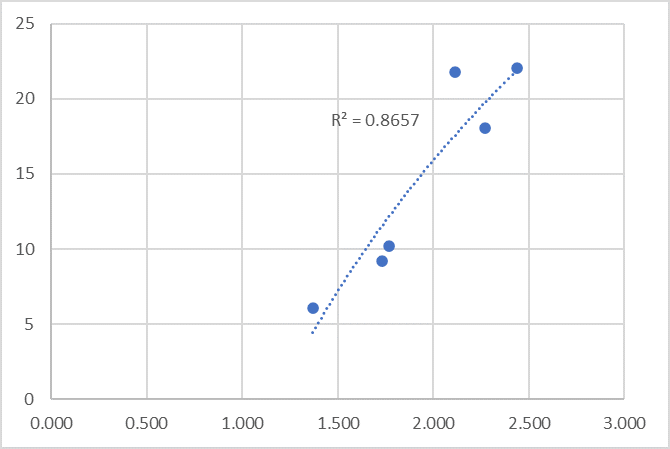
\includegraphics{graph.png}
    \caption{$\text{(L/D)}_{max}$ \text{v/s} $\sqrt{AR_{wet}}$ }
    \label{fig:enter-label}
\end{figure}

\section {Power Loading for Different mission segments}

\subsection {Power Loading for Climb}

\begin{center}
$L/D_{\text{max}} = 14.56067$
\end{center}
\begin{align*}
L/D_{\text{max}} &= \frac{1}{2\sqrt{k \cdot C_{d0}}} \\
C_{d0} &= \frac{1}{4} \left(\frac{L}{D}\right)^2 \cdot k \\
C_{d0} &= 0.018606 \\
\end{align*}
\begin{center}
$W/S = 92.65865 \, \text{N/m}^2$ \\
$V_{\text{stall}} = 11.2 \, \text{m/s}$
\end{center}
\begin{align*}
W/S &= \rho \cdot V_{\text{stall}}^2 \cdot \frac{C_{L_{\text{max, 3D}}}}{2} \\
W/S &= 92.65865 \\
\end{align*}
\begin{center}
$V_{\text{climb}} = 12.69456 \, \text{m/s}$ \\
$V_{\text{takeoff}} = 13.44 \, \text{m/s}$
\end{center}
\begin{align*}
S_{\text{rotation}} &= V_{\text{rotation}} \cdot t_{\text{rotation}} = 20.16 \, \text{m} \\
R_{\text{rotation}} &= \frac{6.96 \cdot V_{\text{takeoff}}^2}{9.81} = 68.99719 \, \text{m} \\
\theta_{\text{climb}} &= \sin^{-1}\left(\frac{S_{\text{rotation}}}{R_{\text{rotation}}}\right) = 13.0995^\circ \\
\end{align*}
\begin{center}
$ROC_{\text{max}} = 2.8770757 \, \text{m/s}$ \\
$\eta_{\text{prop}} = 0.8$
\end{center}
\begin{align*}
\frac{P}{W}_{\text{climb}} &= \frac{ROC_{\text{max}} + \sqrt{\frac{2 \left(\frac{W}{S}\right) \cdot \left(\frac{k}{3C_{d0}}\right)^{1/2}}{\rho}}}{\sqrt{\frac{1.155}{L/D_{\text{max}}}}} \\
\frac{P}{W}_{\text{climb}} &= 3.767996 \\
\end{align*}
\newpage
\subsection {Power Loading for Cruise}

\begin{center}
$V_{\text{cruise}} = 17 \, \text{m/s}$
\end{center}
\begin{align*}
\frac{T}{W}_{\text{cruise}} &= \frac{1}{(L/D)_{\text{cruise}}} = 0.068678 \\
\frac{P}{W}_{\text{cruise}} &= \frac{T}{W}_{\text{cruise}} \cdot V_{\text{cruise}} = 1.167529 \\
\frac{P}{W}_{\text{cruise}} &= 1.167529 \\
\end{align*}

\subsection {Power Loading for Descent}

\begin{center}
$V_{\text{approach}} = 14.56 \, \text{m/s}$ \\
$V_{\text{flare}} = 13.776 \, \text{m/s}$
\end{center}
\begin{align*}
\theta_{\text{descent}} &= \sin^{-1}\left(\frac{S_{\text{flare}}}{R_{\text{flare}}}\right) = 11.52162^\circ \\
V_{\text{cruise to descent}} &= V_{\text{cruise}} \cdot \cos(\theta_{\text{descent}}) = 16.65 \, \text{m/s} \\
V_{\text{average}} &= \frac{V_{\text{cruise to descent}} + V_{\text{approach}}}{2} = 15.605 \, \text{m/s} \\
D_{\text{descent}} &= D_{\text{cruise}} \cdot \cos(\theta_{\text{descent}}) = 4.520132 \, \text{N} \\
P_{\text{descent}} &= D_{\text{descent}} \cdot V_{\text{average}} = 70.53665 \, \text{W} \\
\end{align*}
\begin{center}
$\frac{P}{W}_{\text{descent}} = 1.087755$
\end{center}
\subsection {Power Required for Climb}

\begin{align*}
\frac{P}{W}_{\text{climb}} &= 3.767996 \\
P_{\text{climb}} &= \frac{P}{W}_{\text{climb}} \cdot W \\
&= 3.767996 \times 64.84 \\
&= 244.63 \, \text{W}
\end{align*}

\subsection {Power Required for Cruise}

\begin{align*}
\frac{P}{W}_{\text{cruise}} &= 1.167529 \\
P_{\text{cruise}} &= \frac{P}{W}_{\text{cruise}} \cdot W \\
&= 1.167529 \times 64.84 \\
&= 75.70 \, \text{W}
\end{align*}

\subsection {Power Required for Descent}

\begin{align*}
\frac{P}{W}_{\text{descent}} &= 1.087755 \\
P_{\text{descent}} &= \frac{P}{W}_{\text{descent}} \cdot W \\
&= 1.087755 \times 64.84 \\
&= 70.52 \, \text{W}
\end{align*}

\subsection {Power Required for Loiter}

Since we have assumed that loitering would be done in cruise conditions, we will take all cruise condition values and calculate the power required for loitering.

\begin{align*}
\frac{P}{W}_{\text{loiter}} &= 1.167529 \\
P_{\text{loiter}} &= \frac{P}{W}_{\text{loiter}} \cdot W \\
&= 1.167529 \times 64.84 \\
&= 75.70 \, \text{W}
\end{align*}

The total power required is the sum of the powers required for climb, cruise, descent, and loiter:

\[
\text{Total Power Required} = P_{\text{climb}} + P_{\text{cruise}} + P_{\text{descent}} + P_{\text{loiter}}
\]
\[
= 244.63 + 75.70 + 70.52 + 75.70 = 466.55 \, \text{W}
\]

Given that the power required for takeoff and Landing is negligible, we'll add a tolerance of 20\% to the total power value:

\[
\text{Final Total Power Required} = 466.55 + (0.20 \times 466.55) = 466.55 + 93.31 = 559.86 \, \text{W}
\]
\textbf{The total power required for the UAV is $559.86 \, \text{W}$.}


\subsection {UAV powerplant selection}

\subsubsection {Battery Capacity Calculation}

For each mission segment, we will calculate the energy required in watt-hours by multiplying the power needed for that segment by its endurance time in hours.

\begin{itemize}
    \item Endurance for climb = 2 minutes = 0.0333 hours
    \item Endurance for cruise = 12 minutes = 0.2 hours
    \item Endurance for loiter = 10 minutes = 0.1667 hours
    \item Endurance for descent = 2 minutes = 0.0333 hours
    \item Endurance for takeoff and landing = 4 minutes = 0.0667 hours
\end{itemize}

\begin{align*}
\text{Energy for climb} &= P_{\text{climb}} \times \text{Endurance for climb} \\
&= 244.63 \times 0.0333 \\
&= 8.15 \, \text{Wh} \\
\\
\text{Energy for cruise} &= P_{\text{cruise}} \times \text{Endurance for cruise} \\
&= 75.70 \times 0.2 \\
&= 15.14 \, \text{Wh} \\
\\
\text{Energy for loiter} &= P_{\text{loiter}} \times \text{Endurance for loiter} \\
&= 75.70 \times 0.1667 \\
&= 12.61 \, \text{Wh} \\
\\
\text{Energy for descent} &= P_{\text{descent}} \times \text{Endurance for descent} \\
&= 70.52 \times 0.0333 \\
&= 2.35 \, \text{Wh} \\
\\
\text{Energy for takeoff and landing} &= (\text{Final Total Power Required} \times 1.20) \times \text{Endurance for takeoff and landing} \\
&= (559.86 \times 1.20) \times 0.0667 \\
&= 44.45 \, \text{Wh} \\
\end{align*}

The total energy required is the sum of energies for all mission segments:

\[
\text{Total Energy Required} = 8.15 + 15.14 + 12.61 + 2.35 + 44.45 = 82.7 \, \text{Wh}
\]

To calculate battery capacity, we'll use the formula:

\[
\text{Capacity (mAh)} = \frac{\text{Energy Required (Wh)} \times \text{Flight Time (hours)}}{\text{Voltage (V)}} \times 1000
\]

Now, let's assume a typical lithium-ion battery voltage of 14.8V for calculation purposes.

\begin{align*}
\text{Battery Capacity} &= \frac{82.7 \times 1}{14.4} \times 1000 \\
& = 5587.83 \, \text{mAh}
\end{align*}

So, the total battery capacity required for the aircraft is approximately $22351 \, \text{mAh}$.

\subsubsection{Battery and Motor Selection}

\subsubsection{Battery Selection}

To meet the power requirements with a tolerance of 1000 mAh, we have selected a MaxAmps Lithium Polymer (LiPo) battery with a capacity of 6500mAh operating at a voltage of 14.8V.

\begin{figure}[h]
    \centering
    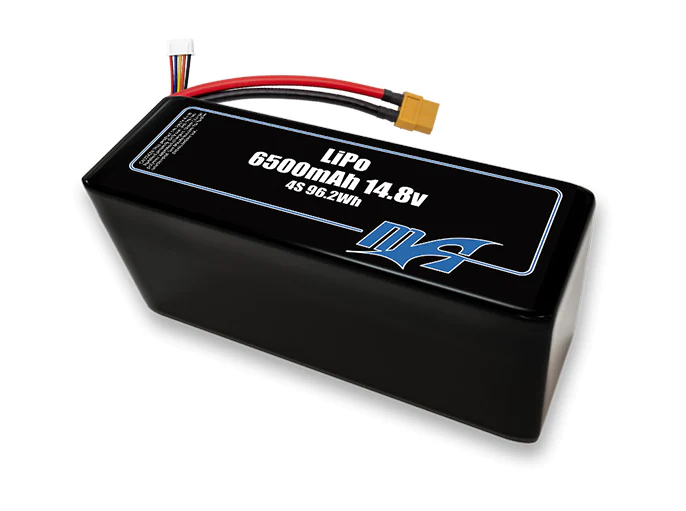
\includegraphics[width=0.7\textwidth]{LIPO.jpg}
    \caption{LiPo Battery}
    \label{fig:battery}
\end{figure}

\begin{table}[h]
    \centering
    \caption{MaxAmps Lithium Battery Specifications}
    \begin{tabular}{|l|l|}
    \hline
    \textbf{Specification} & \textbf{Value} \\ \hline
    Brand & MaxAmps Lithium Batteries \\
    Capacity & 6500mAh \\
    Maximum Voltage & 16.8V \\
    Minimum Voltage & 12V \\
    Recommended Landing Voltage (Air) & 14V \\
    Recommended Cut-off Voltage (Ground) & 12.8V \\
    Chemistry & Lithium-Polymer (LiPo) \\
    Maximum Continuous Discharge & 149.5A \\
    Maximum Charge Current & 32.5A \\
    Watt Hours & 96.2Wh \\
    Energy Density & 151 Wh/kg \\
    Main Lead Length (Custom lengths available) & 5.5" (140mm) \\
    Balance Lead Length (Custom lengths available) & 5.5" (140mm) \\
    Length & 5.43" (138mm) \\
    Width & 1.77" (45mm) \\
    Height & 1.88" (48mm) \\
    Weight & 22.54oz (639g) \\ \hline
    \end{tabular}
\end{table}

\subsubsection{Motor and Propeller selection}

We have selected AT 2317 Long Shaft KV 1440 Motor with APC 8x6 propeller to meet the above calculated power requirements and voltage capacity. All the specifications are mentioned below.

Selecting the right propeller is crucial for efficient performance and optimal thrust generation. We have selected an APC 8x6 propeller that is compatible with our motor.\\

\begin{figure}[h]
    \centering
    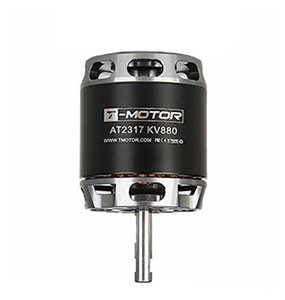
\includegraphics[width=0.3\textwidth]{motorr.jpg}
    \caption{AT2317 LONG SHAFT KV 1440 MOTOR}
    \label{fig:motor}
\end{figure}

\begin{figure}[h]
    \centering
    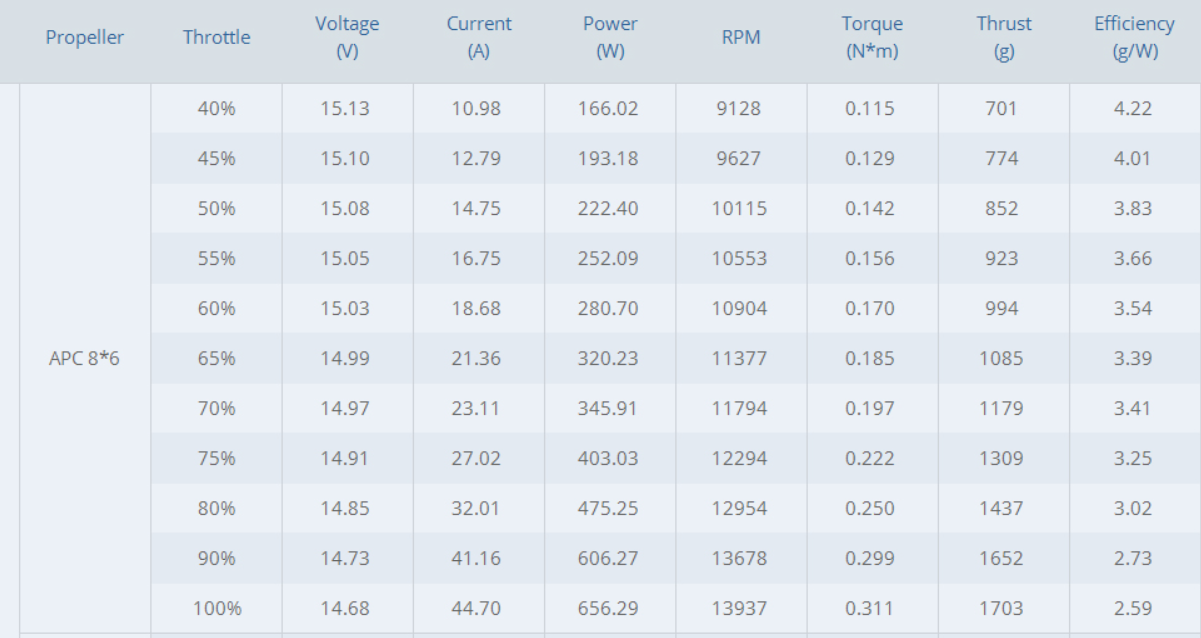
\includegraphics[width=0.8\textwidth]{motor specifications.png}
    \caption{MOTOR SPECIFICATIONS}
    \label{fig:motor_specifications}
\end{figure}


\begin{figure}[h]
    \centering
    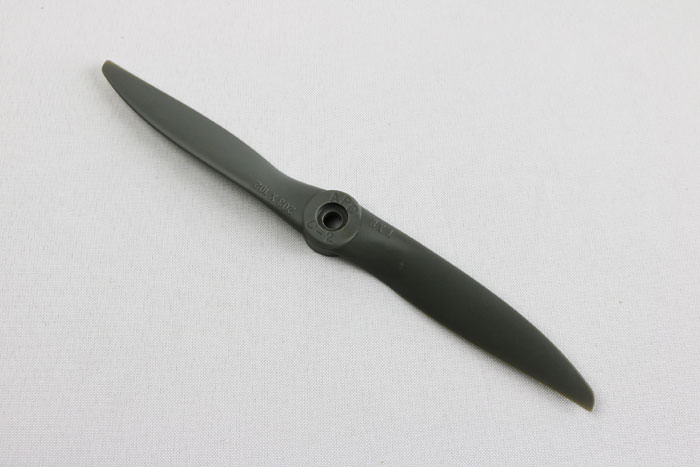
\includegraphics[width=0.5\textwidth]{propeller.jpg}
    \caption{APC 8x6 PROPELLER}
    \label{fig:propeller}
\end{figure}

\begin{figure}[h]
    \centering
    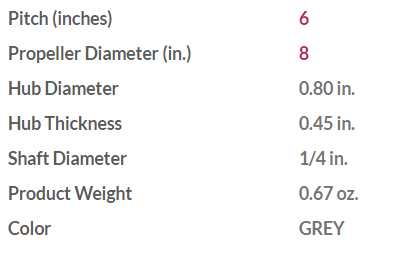
\includegraphics[width=0.6\textwidth]{propeller specifications.png}
    \caption{PROPELLER SPECIFICATIONS}
    \label{fig:propeller_specifications}
\end{figure}

\newpage

\clearpage


\section{Wing Loading}

\subsection{Stall Criteria}
According to \cite{stall1} Stall speed is the minimum speed at which the airplane remains controllable during it's flight for a steady cruise. This is the point where the $C_L$ of the plane is maximum i.e. $C_{L_{\text{max}}}$

At this speed the Angle of attack of the aircraft becomes so large that the flow begins to separate at the top of the airfoil resulting in a drop of lift if we increase the angle of attack beyond that.

\begin{figure}[h]
    \centering
    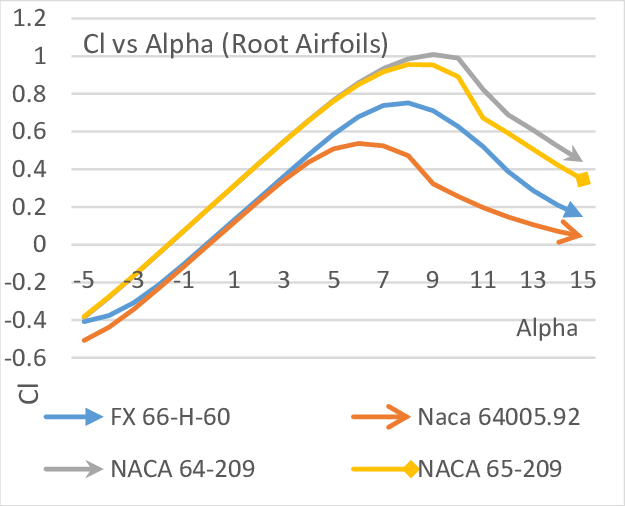
\includegraphics[width=0.6\linewidth]{Extra pics/Cllvsalpha.png}
    \caption{Variation of $C_L$ with angle of attack ref- \cite{stallpic}}
    \label{Variation of $C_L$ with angle}
\end{figure}



\subsubsection{Flaps}
According to \cite{flap} we can decrease the $\text{V}_\text{stall}$ by adding flaps to our airplane. There are different arrangements which we can use for flaps.



\subsection{Cruise}

\subsection{Loiter (Steady Turn)}

\subsection{Climb}
 
\newpage
\textbf{\Huge{Appendix}}
\appendix


\section{References}

\bibliographystyle{IEEEtran}
\bibliography{References}

\vspace{10 pt}

The GitHub account having all the codes can be accessed as: - 

\href{https://github.com/abhijeetmangela/Group_7_design.git}{\text{https://github.com/abhijeetmangela/Group\textunderscore 7\textunderscore design.git}}

\newpage

\section{Changes}

\subsection{Week 2}
\begin{enumerate}
    \item The Data collection part was completely changed.
    \item The general design of the pdf was changed.
    \item More data was added along with a table for better comparison.
    \item Battery performance was estimated.
    \item Weight was estimated.
    \item References were added.
    \item The Mission profile was updated.
    \item Details on mission profile were added.
\end{enumerate}

\subsection{Week 3}
\begin{enumerate}
    \item The Weight estimation was redone
    \item Power was estimated for different phases 
\end{enumerate}

\subsection{Week 4}
\begin{enumerate}
    \item Power calculations were recalculated.
    \item Battery was selected.
    \item Motor and propeller was selected.
\end{enumerate}

\subsection{}
\newpage


\section{Contributions}

\subsection{Week 2}

\subsubsection{Abhijeet Mangela AE21B040}
Wrote full Latek report, Drew the mission profile with Inkscape and Autocad, Empty weight Fraction estimation, and Final weight estimation with Senthil

\subsubsection{Navin Yadav AE23M803}

Data Collection; Literature Survey

\subsubsection{Balamurugan S AE23M009}

Data Collection; Literature Survey

\subsubsection{Samarth R Krishna AE23M032}

Data Collection; Literature Survey

\subsubsection{Senthil B AE23M035}

Detailed Mission Profile; Preliminary Weight Estimation (only iteration); Battery weight estimation.

\subsubsection{Rajendran Anandhu Nair AE23M027}

Data Collection; Literature Survey




\subsection{Week 3}


\subsubsection{Abhijeet Mangela AE21B040}
Changed the Mission Profile, Converted references to BibTeX, Did some cleanup of document, did the Preliminary weight estimate, which was wrong last week, Power estimation for cruise and climb, Linked all files internally in Github for easy connectivity.

\subsubsection{Navin Yadav AE23M803}
The analytical calculation added calculation on latex 

\subsubsection{Balamurugan S AE23M009}
Data Collection; Literature Survey; Max L/D vs Sqrt(Wetted AR) Calculations and Plotting.


\subsubsection{Samarth R Krishna AE23M032}
The analytical calculation added calculation on latex


\subsubsection{Senthil B AE23M035}
Data Collection; Image Processing using ImageJ; Max L/D vs Sqrt(Wetted AR) Calculations and Plotting.


\subsubsection{Rajendran Anandhu Nair AE23M027}
Data Collection; Image Processing using Fusion 360; Report writing for Reference and Wetted areas, Aspect ratios, Coefficient of lift, and Maximum lift-to-drag ratio. 


\section{Current estimates}

\end{document}
